% --------------------------------------------------------------------------------

\begin{exercise}

Sei $A[1, \dots, n]$ ein Feld mit $n$ verschiedenen Zahlen.
Das Paar $(i, j)$ wird Inversion genannt,  wenn $i < j$ und $A[i] > A[j]$ gilt.

\begin{enumerate}[label = (\alph*)]

  \item Welches Feld mit Elementen der Menge $\Bbraces{1, \dots, n}$ besitzt die meisten Inversionen und wie viele Inversionen sind in diesem Feld enthalten?

  \item Welche Beziehung gibt es zwischen der Anzahl von Inversionen im Eingabefeld und der Laufzeit von Insertion-Sort (Einfügesortieren)?

  \item Geben Sie einen Algorithmus an, der die Anzahl von Inversionen in einer Permutation von $n$ Elementen bestimmt und dessen Laufzeit im schlechtesten Fall $\Theta(n \log n)$ ist.
  (Hinweis: Modifizieren Sie Merge-Sort (Sortieren durch Verschmelzen) in passender Weise)

\end{enumerate}

\end{exercise}

% --------------------------------------------------------------------------------

\begin{solution}

Wenn wir die Werte des Datenbereichs auf $\Bbraces{1, \dots, n}$ einschränken, bezeichnet die Anzahl der Inversionen genau die Anzahl der Fehlstände, der durch $A[1, \dots, n]$ induzierten Permutation.

\begin{enumerate}[label = (\alph*)]

  \item Betrachte das Feld $A[1, \dots, n] = [n, \dots, 1]$.
  Klarerweise gilt $\Forall i, j = 1, \dots, n: i < j: A[i] > A[j]$.

  \begin{multline*}
    \implies
    \vbraces
    {
      \Bbraces
      {
        (i, j):
        1 \leq i < j \leq n,
        A[i] > A[j]
      }
    }
    =
    \vbraces
    {
      \Bbraces
      {
        (i, j):
        1 \leq i < j \leq n
      }
    } \\
    =
    \vbraces
    {
      \sum_{j=1}^n
      \Bbraces
      {
        (i, j):
        1 \leq i < j
      }
    }
    =
    \sum_{j=2}^n (j-1)
    =
    \sum_{j=1}^{n-1} j
    =
    \frac{(n - 1) n}{2}
    =
    \begin{pmatrix}
      n \\
      2
    \end{pmatrix}
  \end{multline*}

  \item Für jedes $j = 2, \dots, n$ entspricht die Anzahl der inneren Schleifendurchläufe genau der Anzahl aller $i < j$ mit $A[i] > A[j]$.
  Insgesamt ist die Anzahl der inneren Schleifendurchläufe also genau die Anzahl der Inversionen des Datenfelds.

  \begin{figure}[h!]
    \centering
    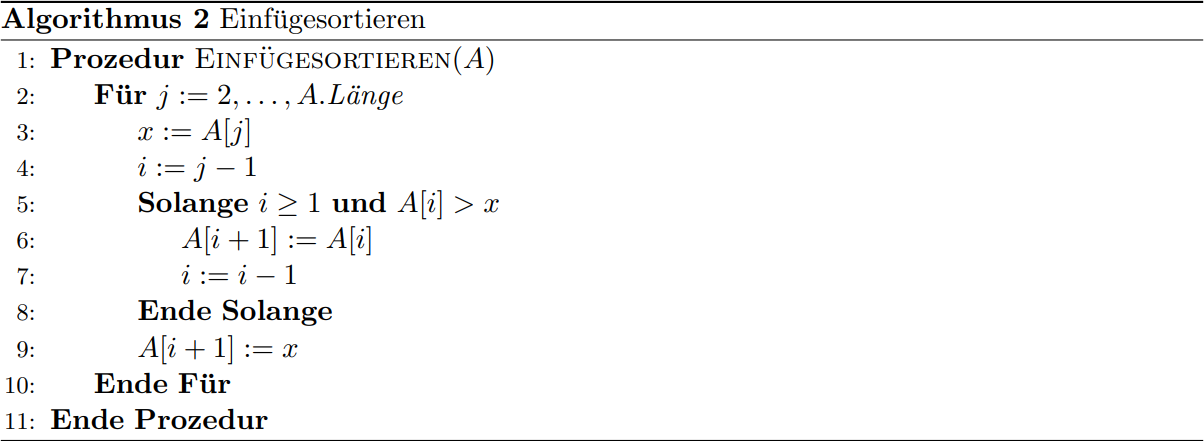
\includegraphics
    [width = 0.75 \textwidth]
    {DGA/DGA - Algorithmus 2 - Einfuegesortieren.png}
    \caption{\cite{DGA}}
  \end{figure}

  \item Wir adaptieren den Verschmelzen-Algorithmus für unsere Zwecke.

  \begin{flalign*}
     1&: \textbf{Prozedur}~ \textsc{Inversions-Verschmelzen} (A, B) \\
     2&: \quad \text{Sei $C$ ein neues Datenfeld  der Länge } A.\textit{Länge} + B.\textit{Länge} \\
     3&: \quad i := 1 \\
     4&: \quad j := 1 \\
     5&: \quad n := 0 \\
     5&: \quad \textbf{Für}~ k := 1, \dots, A.\textit{Länge} + B.\textit{Länge} \\
     6&: \quad \quad \textbf{Falls}~ j > B.\textit{Länge} ~\text{oder}~ (i \leq A.\textit{Länge} ~\text{und}~ A[i] \leq B[j]) ~\textbf{dann} \\
     7&: \quad \quad \quad C[k] := A[i] \\
     8&: \quad \quad \quad \quad i := i + 1 \\
     9&: \quad \quad \textbf{Sonst}~ \\
    10&: \quad \quad \quad C[k] := B[j] \\
    11&: \quad \quad \quad n := n + A.\textit{Länge} - i + 1\\
      &: \quad \quad \quad \implies \text{Wenn}~B[j]<A[i]~\text{dann auch für}~A[i+1],...,A[A.\textit{Länge}] \\
    12&: \quad \quad \quad \textbf{Ende Falls} \\
    13&: \quad \quad \quad j := j + 1 \\
    14&: \quad \quad \textbf{Ende Falls} \\
    15&: \quad \textbf{Ende Für} \\
    16&: \quad \textbf{Antworte}~ C, n \\
    17&: \textbf{Ende Prozedur}
  \end{flalign*}

  Jetzt müssen nur noch im Hauptteil von Merge-Sort die $n$ aufaddiert werden und man erhält zusätzlich zur Sortierung die Anzahl der Fehlstände mit Laufzeit $\Theta(n \log n)$ im Worst-Case.

  \begin{flalign*}
   1&: \textbf{Prozedur}~ \textsc{VInversionszähler} (A) \\
   2&: \quad \textbf{Falls}~ A.\textit{Länge} = 1\\
   3&: \quad \quad \textbf{Antworte}~ A, 0 \\
   4&: \quad \quad \textbf{Ende Falls} \\
   5&: \quad \textbf{Sonst} \\
   6&: \quad \quad m := \left\lceil \frac{A.\textit{Länge}}{2} \right\rceil \\
   7&: \quad \quad L := A[1, \dots, m] \\
   8&: \quad \quad R := A[m+1, \dots, A.\textit{Länge}] \\
   9&: \quad \quad L^\prime, n_L := \textsc{VInversionszähler}(L) \\
  10&: \quad \quad R^\prime, n_R := \textsc{VInversionszähler}(R) \\
  11&: \quad \quad C, n = \textsc{Inversions-Verschmelzen}(L^\prime, R^\prime) \\
  12&: \quad \quad \textbf{Antworte}~ C, n_L + n_R + n \\
  13&: \quad \textbf{Ende Falls} \\
  14&: \textbf{Ende Prozedur}
  \end{flalign*}

\end{enumerate}

\end{solution}

% --------------------------------------------------------------------------------
